\chapter{SYSTEM ARCHITECTURE AND METHODOLOGY}

\section{Block Diagram}

The process of converting a handwritten circuit diagram into a structured netlist involves a series of coordinated steps, each step feeding into the next, designed to detect, extract, and represent pictorial information in a machine-readable format and then using this data for simulation and schematic generation.

\begin{figure}[H]
    \centering
    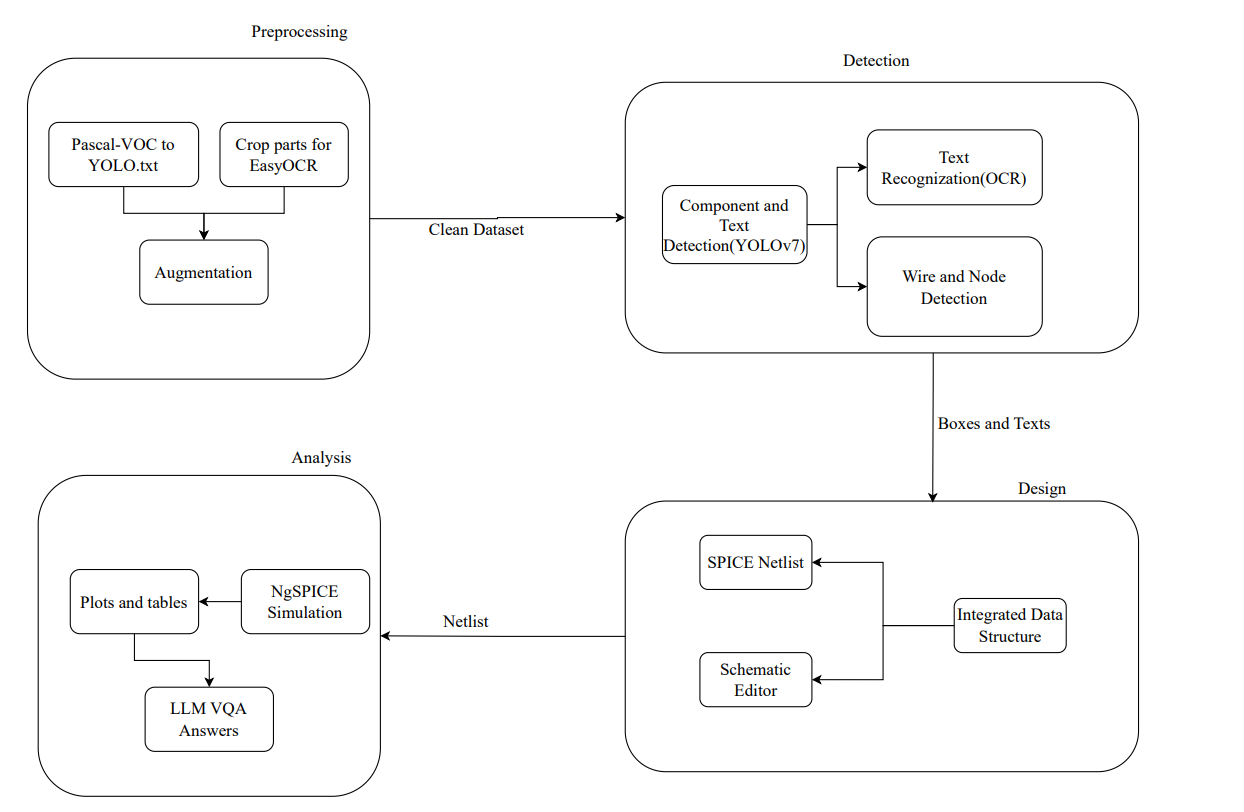
\includegraphics[width=\textwidth]{src/images/figures/block_diagram.png}
    \caption{Block Diagram of the CIRCUITRON System}
    \label{fig:block-diagram-circuitron}
\end{figure}

The high-level architecture of the CIRCUITRON system is visualized in the block diagram in Figure~\ref{fig:block-diagram-circuitron}. Each step involved in the hand-drawn image to simulation-ready schematic pipeline is elaborated as follows.

\subsection{Preprocessing}

At first, the circuit information (components, component values, units, wire intersection, etc.) needs to be extracted out from the hand-drawn image. Appropriately fine-tuned ML and DL models are to be used for each of these steps which will be elaborated on in later subsections. However, for any sort of detection to happen, the image needs to first be pre-processed. Preprocessing for this not only includes image manipulation tasks but also conversion of the dataset annotations into appropriate formats to maintain compatibility with the component detection and text recognition models. The dataset of choice is in the Pascal VOC format which is incompatible with the models used in the pipeline and hence need to be converted. 

Furthermore, image preprocessing, which includes steps like thresholding, contrast and brightness enhancement (for improved clarity) is a vital step in readying the dataset for training any and all models. However, geometric augmentations, especially rotation, is not appropriate for this project.

Among the various available preprocessing techniques, the ones have been selected with careful consideration of the type of images available in the dataset as well as the models in use. Besides image manipulation, preprocessing also includes splitting the dataset into training, validation and testing subsets as appropriate.

\subsection{Circuit Component Detection}

A preliminary yet critical step in the project pipeline is the accurate detection of circuit components from hand-drawn schematic images. This is addressed using a real-time object detection algorithm which is capable of identifying and localizing multiple electronic components (such as resistors, diodes, etc.) directly within the image. YOLO algorithm, the YOLOv7 model, specifically, has been selected for the component detection needs of this project. It is to be noted that text, as a generic collection of letters, numbers, and special characters is also considered a component in this context.

\gls{yolo} (You Only Look Once) is a real-time object detection algorithm known for speed and efficiency. YOLO frames object detection as a single regression problem, straight from image pixels to bounding box coordinates and class probabilities. This model works as follows: first, dividing the image into an $S \times S$ grid. Each grid cell is responsible for detecting objects whose centre falls within it. For each cell, a number of bounding boxes and their corresponding confidence scores (which represents the accuracy of the box and whether the box contains an object) are predicted. Each predicted bounding box includes the coordinates of the box centre relative to grid cell, represented by $(x,y)$, the width and height relative to the whole image, represented by $(w,h)$ and the confidence score $C$ given as:

\begin{equation}
C = P(\text{object}) \cdot \text{IoU}
\label{eq:yolo-confidence-score}
\end{equation}

where $P(\text{object})$ denotes the probability of an object being inside the box, and \gls{iou} is the Intersection over Union between the predicted box and the ground truth box.

Additionally, for each box, class probabilities are predicted as:

\begin{equation}
\text{Class Score} = P(\text{class } i \mid \text{object}) \cdot C
\label{eq:yolo-class-score}
\end{equation}

This allows the model to classify which object exists in each box and once the predictions are made, \gls{nms} is applied to discard less-relevant overlapping boxes.

Based on similar fundamental working principle, several iterations (versions) of YOLO have been introduced and popularized among which YOLOv7 is the YOLO model of choice for this project.

\begin{figure}[H]
    \centering
    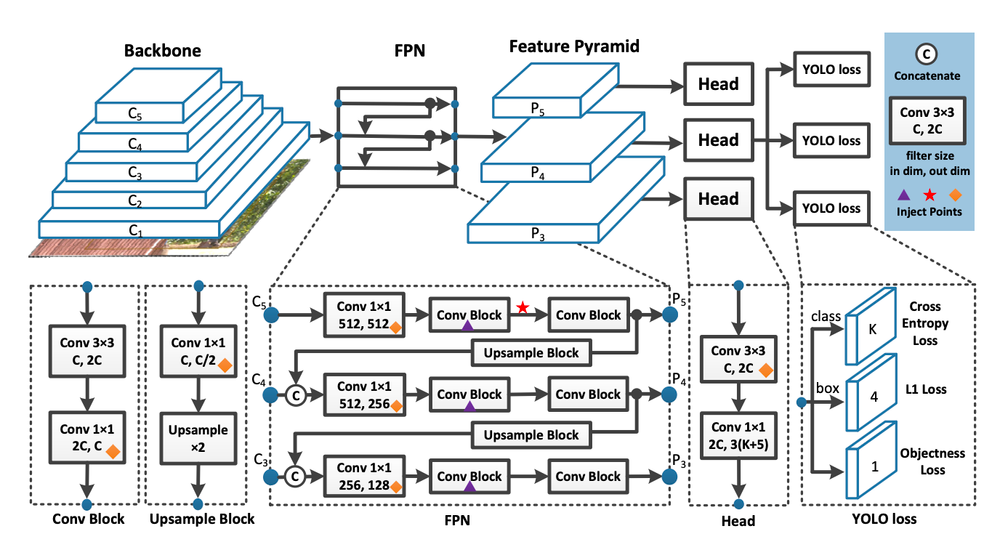
\includegraphics[width=\textwidth]{src/images/figures/yolov7_architecture.png}
    \caption{Architecture of YOLOv7}
    \label{fig:yolov7-architecture}
\end{figure}

Figure \ref{fig:yolov7-architecture} \cite{solawetz2024yolov7} shows the three primary modules of YOLOv7 architecture: Backbone, Neck, and Head, all with their own functions. The CSP-based SPPF backbone extracts essential features from input images. The neck is a PAN which combines features extracted by the backbone and passes them to the head for detection. The head predicts bounding box coordinates, confidence scores, and class probabilities for all the detected objects in a given image.

Prediction of the bounding box coordinates is done through anchor-based regression such that the final box $B=(x,y,w,h)$ is worked out relative to the anchor box as follows:
    
    \begin{equation}
    x = \sigma(t_x) + c_x
    \label{eq:bbox-x}
    \end{equation}
    
    \begin{equation}
    y = \sigma(t_y) + c_y
    \label{eq:bbox-y}
    \end{equation}
    
    \begin{equation}
    w = p_w \cdot e^{t_w}
    \label{eq:bbox-w}
    \end{equation}
    
    \begin{equation}
    h = p_h \cdot e^{t_h}
    \label{eq:bbox-h}
    \end{equation}
    
    where $(t_x, t_y, t_w, t_h)$ are the predicted offsets, $(c_x, c_y)$ is the top-left corner of the grid cell, and $(p_w, p_h)$ are the dimensions of the anchor box.
    
    YOLOv7 runs auto-augmentation features (mosaic augmentation, HSV shifts, crops, rescaling, etc.) during training along with other features to increase dataset variability. Built-in early stopping is also there; if the validation loss (a mix of box loss, objectness loss, and classification loss) plateaus for a set number of epochs, training cuts off on its own to avoid overfitting.

\subsection{Recognition of Component Values}

In order to generate a complete and simulation-ready netlist, it is essential to not only detect the components themselves but also to extract their associated parameter values, which are generally annotated near the components in the circuit diagram. Thus, it becomes essential to integrate Optical Character Recognition (\gls{ocr}) with the object detection pipeline to extract and map these values correctly to the corresponding components.

This involves identifying regions within the circuit image that likely contain text (done by YOLOv7), and then recognizing said texts in order to parse the component values along with their units.

The hand-written text recognition is done using a \gls{crnn}-based \gls{ocr} system, following the design philosophy of Deep Text Recognition Benchmark (DTRB) framework, however minor changes deemed suitable for this project have been made to get the text detection and recognition pipeline.

\begin{figure}[H]
    \centering
    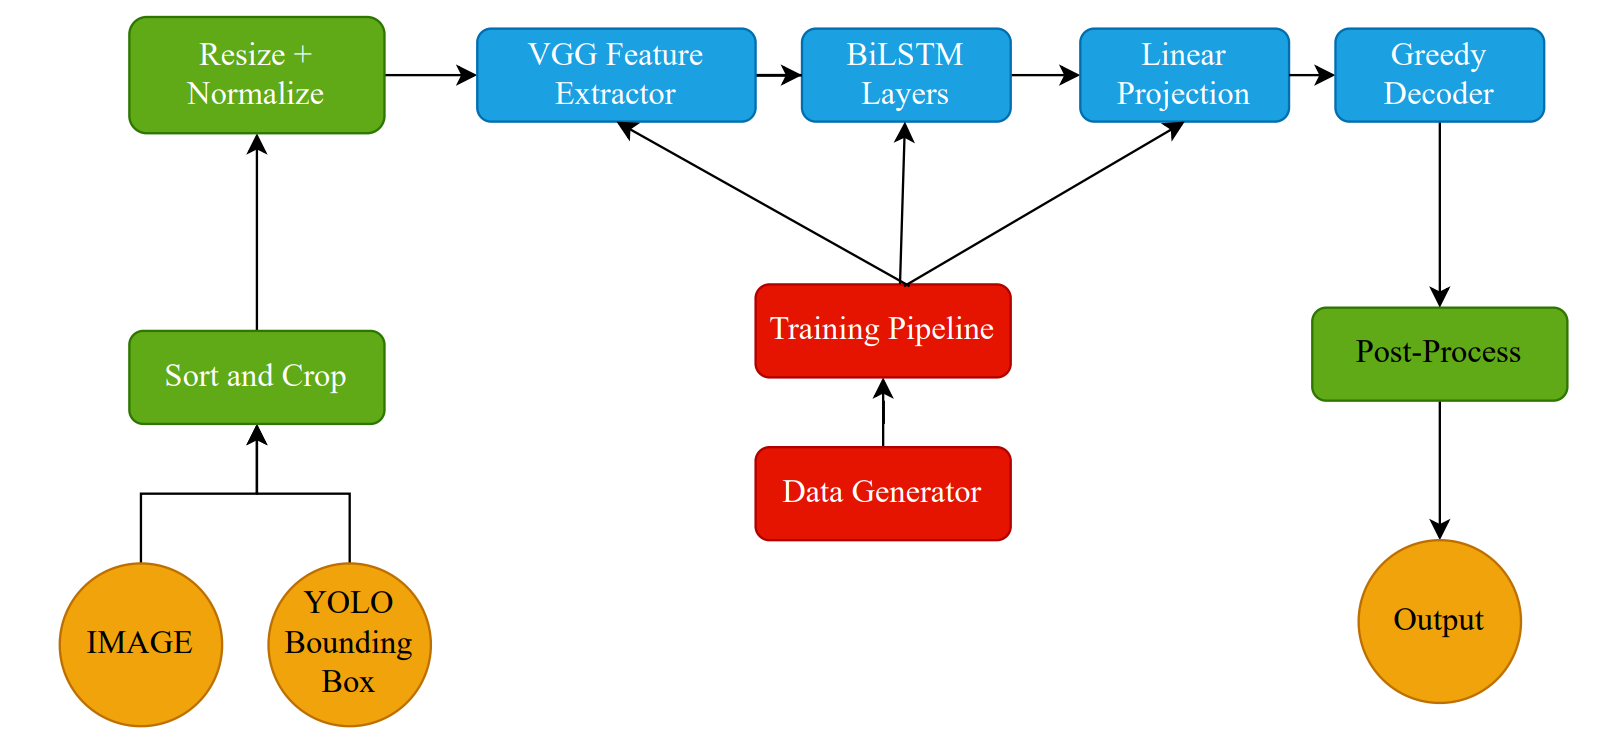
\includegraphics[width=\textwidth]{src/images/figures/easyocr_architecture.png}
    \caption{Text Detection and Recognition Pipeline}
    \label{fig:text-recognition-pipeline}
\end{figure}

YOLOv7 outputs (bounding box information) help segregate textual information (class `0' in the used dataset) which are then cropped, resized (to image height as 64) and normalized for compatibility with text recognition module. This is then passed through to a \gls{crnn} architecture composed of a Convolutional Encoder, Sequence Modeling Engine with Linear Projection, and \gls{ctc} Decoder as shown in Figure \ref{fig:text-recognition-pipeline}.

\textbf{Convolutional Encoder (CNN):} A \gls{cnn} stack (e.g., VGG) transforms input image $I$ from multi-dimensional $\mathbb{R}^{H \times W \times C}$ to feature maps:

\begin{equation}
F = f_{\text{CNN}}(I_i), \quad F \in \mathbb{R}^{H' \times W' \times C}
\label{eq:cnn-encoder}
\end{equation}

\textbf{Sequence Modeling (Bidirectional LSTM):} Each $F$ becomes input to a bidirectional \gls{lstm}, yielding hidden states $h_t$. These hidden states capture context across the text line, allowing modeling of character sequences:

\begin{equation}
\overrightarrow{h_t} = \text{LSTM}_f(F_t, \overrightarrow{h_{t-1}})
\label{eq:bilstm}
\end{equation}

\textbf{CTC Decoder:} A softmax layer projects $h_t$ over the character vocabulary as:

\begin{equation}
p_{t,k} = \frac{e^{W_k h_t + b_k}}{\sum_{k'} e^{W_{k'} h_t + b_{k'}}}
\label{eq:ctc-softmax}
\end{equation}

The probability of sequence $z$ is computed over all alignments:

\begin{equation}
P(z \mid y) = \sum_{\pi: B(\pi)=z} \prod_{t=1}^{T} p_{t,\pi_t}
\label{eq:ctc-probability}
\end{equation}

The \gls{ctc} loss is given by the negative logarithm of $P(z \mid y)$. It enables end-to-end sequence decoding without explicit character bounding boxes.

During inference, greedy decoding strategy is used which selects the most-probable character at each time step while removing blank symbols and collapsing consecutive duplicate characters. The recognized text then needs to be mapped to the appropriate circuit component whose value it represents.

This project includes two separate OCR models for character recognition, the second one being TrOCR (TrOCR-small to be exact) developed by Microsoft, specifically for handwritten text. 

\begin{figure}[H]
    \centering
    \includegraphics[width=\textwidth]{src/images/figures/trocr.png}
    \caption{Architecture of TrOCR}
    \label{fig:trocr-architecture}
\end{figure}

Figure \ref{fig:trocr-architecture} \cite{li2021trocr} shows the encoder-decoder model (with pre-trained image transformer as encoder, and pre-trained text transformer as decoder) completing the basic architecture of TrOCR. The image transformer obtains the representaton of image patches, and likewise, with the help of visual features and previous predictions, the text transformer generates the wordpiece sequence.

The process begins with the raw input image, denoted as $x_{img} \in \mathbb{R}^{3 \times H_0 \times W_0}$. The transformer architecture is designed to process sequences rather than raw pixel grids, therefore the image is first resized to a standardized dimension $(H, W)$. 

To format this data for the model, the image is decomposed into a series of $N$ fixed-size square patches. For $P$ as the patch side length, the total number of patches is given as:
\[
N = \frac{HW}{P^2}
\]

Every patch gets flattened into a vector and then linearly projected into a $D$-dimensional space; $D$ here is the hidden dimension that stays constant across all transformer layers.

A \texttt{[CLS]} token is prepended to the sequence so that global information can be pooled into a single representation. If pre-trained DeiT models are used for initialization, a distillation token gets tacked on as well to help the model learn from a teacher. Transformers on their own have no built-in sense of where patches sit spatially (unlike CNNs), so learnable 1D position embeddings are summed into the patch embeddings to retain absolute positional cues. Viewing the image as a sequence of standalone patches lets the model spread its attention across fine-grained details or the broader layout as needed.

The decoder follows the standard transformer decoder blueprint for producing the final text sequence. It mirrors the encoder's stacked-layer design, though an encoder-decoder attention block is wedged in between the self-attention and feed-forward portions. Queries in this block come from the decoder's own internal state, and keys along with values are drawn from the encoder output. That arrangement lets the decoder zero in on whichever visual features matter most at each generation step.

A self-attention mask keeps the model from peeking at future tokens while training. The output at any position $i$ therefore depends solely on the tokens before it. Hidden states from the decoder pass through a linear layer sized to the vocabulary $V$, and the resulting probability distribution over the vocabulary comes from the softmax function:
    \[
    \sigma(h_{ij}) = \frac{e^{h_{ij}}}{\sum_{k=1}^{V} e^{h_{ik}}}
    \]
At inference time, beam search is used to explore the probability space and land on the most probable character sequence.

\subsection{Wire Detection}

Junction points picked up by the object detection model act as structural anchors for figuring out how the circuit is wired. The detected junction coordinates are first converted from the normalized values into pixel coordinates. At this stage, which junctions are actually connected is still unknown, so each pair of junctions needs to be examined to see which ones could form wire connections. For each junction pair, the displacement and the angle between them is computed and since most circuit diagrams use only horizontal and vertical wires, diagonal pairs are discarded. The remaining pairs of junctions are then forced into perfectly horizontal or vertical segments. As the detection is never perfectly accurate, the wire endpoints are snapped to a uniform grid in order to align slightly-off wires. Segments that lie on the same line and overlap with each other are also merged. After these corrections, we obtain a clean set of wire segments that accurately reflects the wiring drawn in the diagram in strictly horizontal and vertical planes. This is a limitation that is fixed by the BFS-based algorithm, discussed in later sections. 

\subsection{Terminal Point Detection}

After detecting components (through YOLO) and wires, the exact points where they connect are still unknown. The junction points detected earlier give a good starting point for locations of wire connections, since they include wire endpoints and intersections.

To find the actual terminals, we check where horizontal or vertical wire segments enter (or touch) the component bounding boxes. Whenever a wire intersects with a bounding box, calculated using self-defined line-rectangle intersection rules, we treat that crossing as a terminal point. These terminal points reveal which wires are connected to which components. This information is then used to build the circuit graph and to display the connections correctly in the frontend.All components of the project (CircuitJS-compatible text file generation, schematic editing, etc.) build on this representation downstream.

\subsection{Integration Algorithm}

From the individual outputs from each of the aforementioned modules, the task is now to generate a structured \gls{json} representation of the circuit which has is to be used to generate a corresponding CircuitJS-compatible text file and also contribute in the schematic generation further down the line.

The integration between all these different outputs, in a simplistic form, would consist of the following steps:

\begin{itemize}
    \item Get a list of components and their corresponding bounding box coordinates (from YOLOv7).
    
    \item Get a list of text data and their corresponding bounding box coordinates (from \gls{ocr}).
    
    \item Map the component to the corresponding component value (text) based on the minimum Euclidean distance between a particular component and texts on the circuit.
    
    \item Once the terminals are determined based on the bounding boxes, match those terminal points to the nearest nodes in the circuit.
    
    \item Store the accumulated information in a \gls{json} file.
\end{itemize}

\subsection{CircuitJS-compatible Text File Generation}

A circuitJS-compatible text filedescribes the connections between components in an electronic circuit. It acts as a blueprint, specifying which components are connected and how, without detailing the physical layout or specific component placement.

It is a text-based representation of an electrical circuit used for simulation by the CircuitJS engine. It provides all the necessary information about the components, their connections, and their electrical properties, enabling analysis such as transient response, DC/AC sweep, or frequency domain behavior.

The text file serves as input to a circuit simulation engine, which then performs numerical computations to evaluate how the circuit behaves under specified conditions.

For each component, this text file contains the information about its name, the nodes it is connected to on either side and the component's parameters or model (if necessary).

After the \gls{json} file with abundant information about the components, their values, and the nodes they are connected to is generated, the next step is to convert said \gls{json} file into a CircuitJS-compatible file (a \texttt{.txt} file which follows the appropriate conventions).

\subsection{Digital Schematic Generation}

The \gls{json} file built by integrating all the information about the hand-drawn circuit is to be manipulated through different JavaScript libraries to generate a digital, editable schematic of the circuit. As briefly discussed in the Requirements section, react-draggable is used to map each component in \gls{json} to a visual block (a symbol for the component as given by the KiCad symbol library). For each component, a graphical symbol needs to be rendered at a certain position and connection lines need to be drawn between the terminals and node positions. A rough pseudocode for the same is as follows:

\begin{algorithm}
\caption{Frontend Circuit Rendering}
\label{algo:frontend-rendering}
\begin{algorithmic}
\Require Circuit \gls{json} description $J$
\Ensure Rendered circuit schematic
\For{all component $c \in J.\text{components}$}
    \State Draw schematic symbol of type $c.\text{type}$ at position $c.\text{position}$
    \State Attach text label $c.\text{value}$ near component position
\EndFor
\For{all connection $k \in J.\text{connections}$}
    \State Retrieve terminal position from $k.\text{from}$ and terminal index
    \State Retrieve node position from $k.\text{node}$
    \State Draw wire between terminal and node positions
\EndFor
\State \Return Rendered schematic
\end{algorithmic}
\end{algorithm}

\subsection{Backend Development}

The backend has been constructed using Next.js and FastAPI, functioning as the core middleware responsible for routing, and processing the system's \gls{ml} pipeline and user interactions. All the endpoints are based on REST API which ensures the frontend and backend can communicate statelessly.

When the user uploads a circuit image through the UI, it reaches the upload endpoint (say /upload) which first saves it to temporary storage (may be local storage of browser). From there, a chain of processes which are involved in the project pipeline are executed. The preprocessing steps, for both component detection and text recognition are first executed, and then, in a sequential fashion, the models as well. The tasks like deleting components, adding wires, changing values, resizing, rotating components, etc. are handled by CircuitJS and the role of backend in this case is just to be the facilitator for this, for communication and temporary storage.

\subsection{LLM Integration}

Using the publicly available Deepseek v3.1 API, the project is elevated from simple circuit manipulation tool to one capable of auto-analysis. The LLM has context about the uploaded image as well as the associated netlist or CircuitJS text file using which it can produce accurate responses to user's queries (prompts) related to their circuit. It can expain the reason for placement of a particular circuit component or why a particular value has been used, and much more.

\section{Line Detection}

To address the limitations of the junction-based wire detection algorithm which used only horizontal and vertical classification, Multi-Head BFS-based wire detection and generation algorithm was built. However, both approaches were extensively used and tested, and hence both have been explained in upcoming sections. 

\subsection{Line Detection via Horizontal and Vertical Classification}

For this approach, the junction points detected by the component detection model (YOLOv7 at the end, but also other YOLO models during testing) are needed first. The coordinates given by YOLO falls under the range $[0,1]^2$, so they need to be denormalized into pixel space using $\mathcal{N}^{-1}(x_n, y_n) = (W \cdot x_n,\; H \cdot y_n)$. Then, junction pairs are formed for processing. Every junction is paired up with every other junction. For a given pair $(\mathbf{j}_i, \mathbf{j}_k)$, the displacement between them and angular orientation is needed. For this, we calculate the displacement vector using $\mathbf{d} = \mathbf{j}_k - \mathbf{j}_i$ and the angular orientation $\tilde{\theta}$ using arctangent.

Using $\tilde{\theta}$, the junction pairs are classified with $18^\circ$ tolerance.
\begin{itemize}
    \item \textbf{Horizontal:} $\tilde{\theta} \in [0^\circ, 18^\circ] \cup [162^\circ, 198^\circ] \cup [342^\circ, 360^\circ]$
    \item \textbf{Vertical:} $\tilde{\theta} \in [72^\circ, 108^\circ] \cup [252^\circ, 288^\circ]$
    \item \textbf{Diagonal (rejected):} remaining angles
\end{itemize}

Those pairs which are not rejected (i.e those with diagonal lines assumed between them) are projected onto perfectly horizontal or vertical lines. This is done since hand-drawn wire lines may be slightly jagged or imperfect in other ways. These lines are then snapped to a 16-pixel grid by consolidating overlapping segments which can be considered collinear (provided that they have the same angular orientation and fall within the grid tolerance). To determine where wires are actually connected to the components, intersection of each bounding box and any horizontal or vertical wire it touches is calculated.

In this approach, the wire connections are simply guessed based on the junction points, without taking into account the actual wire paths in the circuit. Those junction pairs which are completely unrelated but are axis-aligned may end up being connected. All issues in this step are inherited by terminal detection step as well, eventually leading to completely inaccurate results.

\subsection{Line Detection via Path Finding}
\label{sec:line-detection-pathfinding}

The geometric approach's shortcomings called for something fundamentally different, so a skeleton-based path-finding method was put together. Instead of guessing connections from junction positions, this pipeline works straight on skeletonized circuit images, following the actual wire paths. At its core sits a Multi-Head Breadth-First Search (BFS) algorithm. The whole process splits into two stages, endpoint detection and graph construction.

\textbf{Endpoint Detection:} How endpoints are found depends on what class the object belongs to. Junction points (class 1) get a single endpoint: the bounding box center $(x_c, y_c)$ is snapped to whichever skeleton pixel sits closest within an expanded search region (margin = 8 pixels). Components (class 2+) need two endpoints instead. Skeleton pixels lying on or near the bounding box border are scanned, with preference given to true topological endpoints (degree = 1). The pair with the greatest separation wins.

\textbf{Graph Construction via Multi-Head BFS:} A graph gets built with detected endpoints as nodes and skeleton connectivity supplying the edges. Every node claims a disk of radius $r$, and a \texttt{node\_id\_map} is precomputed so that each pixel knows which node owns it (or carries $-1$ if none does). BFS launches from each source node: the queue starts with skeleton pixels sitting at the disk boundary and crawls along the skeleton through 8-connectivity. The moment a pixel owned by some other node $j$ turns up, the edge $(i, j)$ is logged and that particular branch stops. Once the full graph is in place, self-edges get pruned. These are edges connecting two endpoints of the same bounding box, and stripping them out guarantees that only inter-object connections survive.

\textbf{Advantages over horizontal/vertical classification:} Because path-finding follows the actual wire paths visible in the image, phantom connections vanish. Wire orientation ceases to matter altogether; horizontal and vertical wires get handled just the same as diagonal ones. Wire detection and terminal detection collapse into one graph-construction step. Scaling is linear with skeleton pixel count instead of quadratic with junction count. For all of these reasons, the final deployed system runs on this approach.

\subsection{Crossover Dissolution Algorithm}

Hand-drawn circuit diagrams contain two visually similar yet electrically opposite situations i.e, a \textit{crossover}, where two wires pass over each other without any electrical contact, and a \textit{junction}, where wires genuinely meet. Getting the distinction wrong ruins circuit reconstruction entirely. YOLOv7 flags crossovers as their own class. Multi-Head BFS (Section~\ref{sec:line-detection-pathfinding}) then slots each one in as a single-point graph node, usually connected to four neighboring endpoints that correspond to the two wire segments crossing at that spot. The dissolution algorithm's job is to untangle these nodes into the correct topology.

\textbf{Candidate Identification:} A crossover node must have exactly four neighbors to be eligible for dissolution. Anything with fewer neighbors stays in the graph as a regular junction. This sidesteps problems where the detector mistakenly labels a junction as a crossover, or where a wire happens to dead-end right at the crossing.

\textbf{Direction Vector Computation:} Given a crossover node sitting at position $\mathbf{p}$, a unit direction vector pointing toward each of its four neighbors $\mathbf{n}_k$ is worked out as:
\begin{equation}
    \hat{\mathbf{d}}_k = \frac{\mathbf{n}_k - \mathbf{p}}{\|\mathbf{n}_k - \mathbf{p}\|}
\end{equation}

\textbf{Optimal Pairing via Dot Product:} Four neighbors can be split into two pairs in exactly three ways. Each candidate pairing $\{(\mathbf{n}_a, \mathbf{n}_b),\; (\mathbf{n}_c, \mathbf{n}_d)\}$ receives a score equal to the sum of dot products within its pairs:
\begin{equation}
    S = \hat{\mathbf{d}}_a \cdot \hat{\mathbf{d}}_b + \hat{\mathbf{d}}_c \cdot \hat{\mathbf{d}}_d
\end{equation}
Whichever pairing yields the most negative $S$ wins. A strongly negative score means the paired neighbors sit on roughly opposite sides of the crossover, which is exactly the geometry expected when two wires cross.

\textbf{Geometric Validation:} Before anything gets rewired, both dot products in the chosen pairing have to clear a threshold: $\hat{\mathbf{d}}_a \cdot \hat{\mathbf{d}}_b < -0.7$. Passing this check confirms that each paired neighbor lies within roughly $45^\circ$ of being directly across from the other through the crossover center.

\textbf{Graph Transformation:} When validation succeeds, the crossover node gets ripped out of the adjacency graph. Two fresh edges take its place, each linking one pair of opposite neighbors directly. What was a four-way junction now becomes two independent through-connections, faithfully modeling two wires that happen to cross paths without touching. Should the validation fail, the node simply remains as a junction so that electrical connectivity is preserved.

Once dissolution wraps up, the resulting graph feeds into final circuit assembly. Nodes in this graph stand for component terminals and junctions alongside wire endpoints; edges trace the actual wire paths. Crossover points no longer appear anywhere in the electrical topology.

\section{Use-Case Diagram}

\begin{figure}[H]
    \centering
     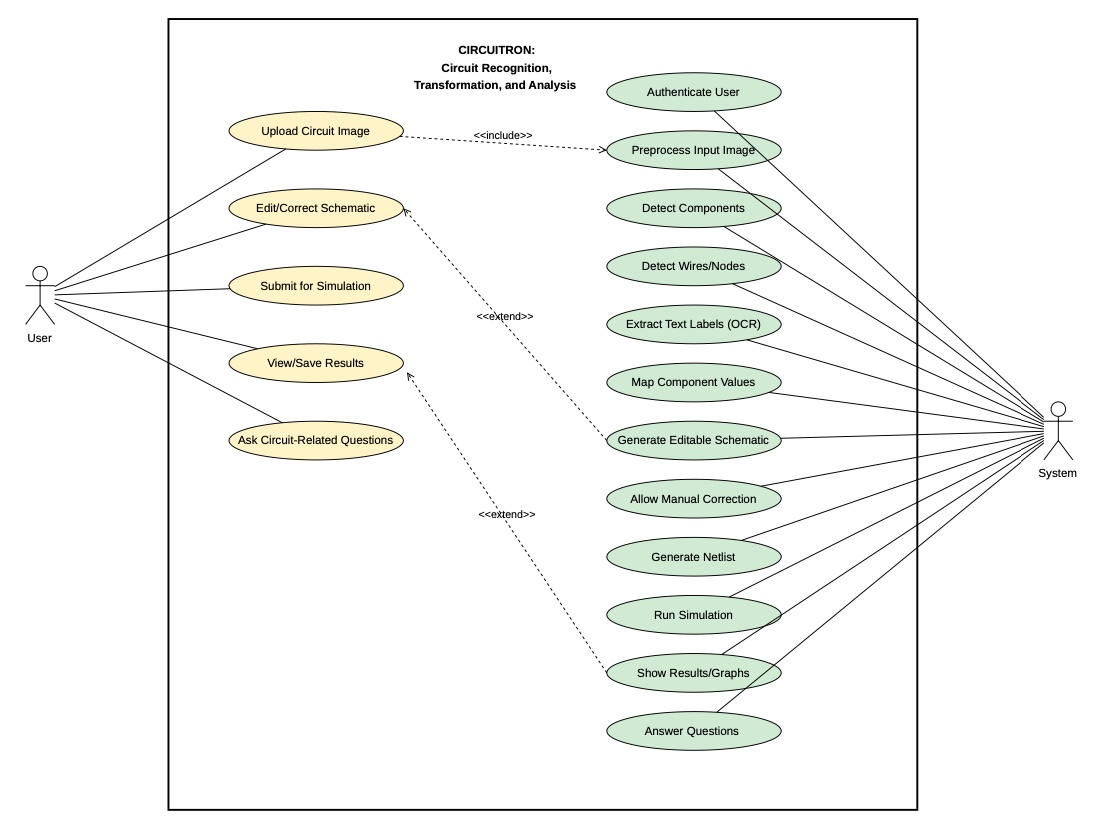
\includegraphics[width=\textwidth]{src/images/figures/use_case_diagram.png}
    \caption{Use-Case Diagram for CIRCUITRON System}
    \label{fig:use-case-diagram}
\end{figure}

Figure~\ref{fig:use-case-diagram} lays out how users interact with the CIRCUITRON system. The primary actor here is the user, whether that happens to be a student, an instructor, or a practicing engineer. Everything kicks off when the user uploads a hand-drawn circuit image.

As soon as the image lands, CIRCUITRON preprocesses it to sharpen clarity. YOLOv7 then picks out the components (e.g., resistors, capacitors) while junction-based wire detection maps out the wires and nodes. \gls{ocr} runs at the same time, pulling text labels (e.g., component values) off the image and pairing them with the right components.

From the parsed circuit structure, an editable schematic gets generated. Users can step in at this point and manually fix any mistakes. Once they are satisfied, the schematic is converted into a CircuitJS-compatible text file and fed into CircuitJS for simulation. Voltage and current graphs come back as the output. An AI assistant is included as well for answering circuit-related questions. This may help in simply clearing up circuit-related questions and concepts, or also help in debugging.

In the diagram, the ``includes'' relationship flags sub-tasks that have to run every time, like component detection and \gls{ocr}. ``Extends'' covers the optional bits, things like manual corrections or AI Q\&A that add value but are not strictly necessary for the core workflow. Taken together, the diagram captures the full scope of what the system can do.

\section{Performance Metrics Expectation}

Even with careful training and fine-tuning, edge cases will slip through. Illegible handwriting or components that look nearly identical can trip up any model. That makes it essential to pin down performance metrics ahead of time so there is a clear threshold for when a model qualifies as ``good-enough.'' Table~\ref{table:performance-metrics} lists the metrics chosen for this project along with the target values; once those targets are hit, training can be halted.

\begin{table}[H]
    \centering
    \caption{Expected Performance Metric Values for Individual Modules}
    \label{table:performance-metrics}
    \begin{tabular}{lcc}
        \toprule
        \textbf{Pipeline Stage} & \textbf{Performance Metric} & \textbf{Target Value/Expectation} \\
        \midrule
        Component Detection & mAP@0.5 & 0.95 \\
        Text Recognition & Character Accuracy & 0.65 \\
        \bottomrule
    \end{tabular}
\end{table}

\subsection{Component Detection Metric}

mAP@0.5 (mean Average Precision at an IoU threshold of 0.5) gauges how accurately the model spots components while getting both the class label and the bounding box right. \gls{ap} is computed per class first, and then averaged across every class. Setting the \gls{iou} threshold at 0.5 means a predicted box counts as correct only when its overlap with the ground truth box reaches at least 50\%.

\begin{equation}
\text{IoU} = \frac{\text{Area of Overlap}}{\text{Area of Union}}
\label{eq:iou-metric}
\end{equation}

When mAP@0.5 is high, it signals that detections are landing accurately and that few components are being missed or mislabeled.

\subsection{Text Recognition Metric}

Character Accuracy tallies how many individual characters in the predicted text line up with the ground truth:

\begin{equation}
\text{Character Accuracy} = \frac{\text{Number of Correct Characters}}{\text{Total Number of Characters in Ground Truth}}
\label{eq:character-accuracy}
\end{equation}

Component values on circuit diagrams ($10k$, $100\Omega$, $1\mu F$, and so on) leave zero room for misreads. Even one wrong character, say confusing `k' with `1', throws off the entire simulation. \gls{ocr} has to nail these consistently, because reliable value-to-component mapping hinges on high character accuracy.

\section{System Flowchart}

\begin{figure}[H]
    \centering
    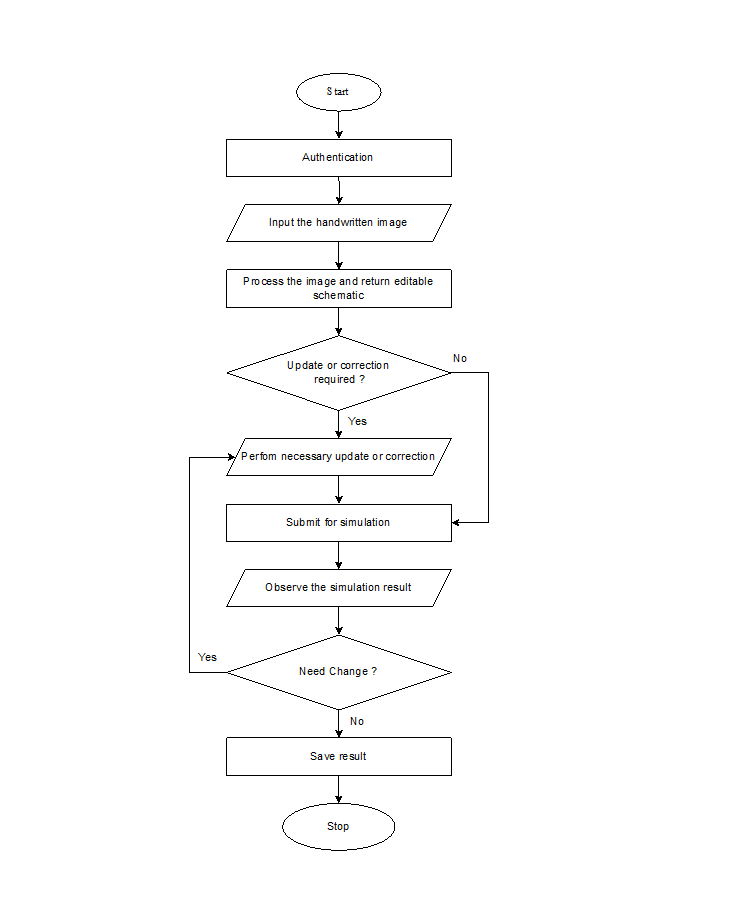
\includegraphics[width=0.85\textwidth]{src/images/figures/flowchart.png}
    \caption{System Flowchart}
    \label{fig:system-flowchart}
\end{figure}

The key architectural modules involved in the working of the system have been demonstrated by the block diagram in Figure~\ref{fig:block-diagram-circuitron}. Now, the flowchart in Figure~\ref{fig:system-flowchart} demonstrates the motions a user needs to go through to use the final product. Once the image of a hand-drawn circuit is uploaded, the system processes the image (internally using the techniques explained in the previous sections) and returns an editable schematic. Any necessary update or correction may be performed if necessary and then the schematic can be submitted for simulation and analysis. Relevant graphs are returned after analysis.

\section{Dataset Analysis}

In order to develop the system using the system for automated circuit diagram understanding, the \gls{cghd} (Circuit Graph Handwritten Diagrams) dataset is used. This dataset provides a comprehensive suite of ground truth annotations tailored to facilitate key computer vision tasks such as object detection, instance segmentation, and text recognition. While additional datasets (such as circuitVQA, Digitize-HCD datasets) may be used to fine-tune the models in the future to achieve even higher values for performance metrics, as of yet, only the \gls{cghd} dataset has been used.

\subsection{Dataset Overview}

The \gls{cghd} dataset comprises 4.99 GB of annotated data spanning over 3,000 raw images. The data is separated into folders named drafters, going from $-1$ through 31, and each drafter folder contains hand-sketches of 12 unique circuit designs, with each circuit drawn twice and captured under four different conditions (varying angles, lighting, and minor distortions), resulting in up to 96 images per drafter. As is convention, the dataset is to be split into (70-10-20)\% of the entire data for training, validation and testing respectively.

\begin{table}[H]
    \centering
    \caption{Summary of Data in the CGHD Dataset}
    \label{table:cghd-summary}
    \begin{tabular}{lr}
        \toprule
        \textbf{Items} & \textbf{Number} \\
        \midrule
        Distinct Circuits & 372 \\
        Raw Images & 3,269 \\
        Bounding Box Annotations & 248,020 \\
        Text String Annotations & 85,417 (93.74\% completeness) \\
        Character Types & 98 \\
        Object Classes & 61 \\
        \bottomrule
    \end{tabular}
\end{table}

Every image is rigorously annotated and the annotations provided per image include:

\begin{itemize}
    \item \textbf{Bounding Boxes (PASCAL VOC format)} for 61 electrical component classes, including resistors, capacitors, transistors, operational amplifiers, and textual elements.
    
    \item \textbf{Text Labels} that indicate component values and identifiers (e.g., ``$10k\Omega$'', ``$C1$'', ``$V$'').
    
    \item \textbf{Instance Segmentation Polygons} (LabelMe JSON format) for pixel-level object outlines.
    
    \item \textbf{Binary Segmentation Maps} that differentiate circuit strokes (foreground) from background artifacts.
    
    \item \textbf{Partial Netlist Files} (in \texttt{.asc} format) for some samples; useful for validating circuit reconstruction.
\end{itemize}

The text annotation coverage is extensive, with labels ranging from single characters (like ``$R$'' or ``$R1$'') to full descriptors (like ``Resistor'', ``Variable Resistor'', etc.).

\subsection{Class-wise Data Statistics}

\begin{table}[H]
    \centering
    \caption{Frequency of Each Class with its Code in the CGHD Dataset}
    \label{table:cghd-classes}
    \begin{tabular}{rll|rll}
        \toprule
        \textbf{Code} & \textbf{Class Name} & \textbf{Count} & \textbf{Code} & \textbf{Class Name} & \textbf{Count} \\
        \midrule
        1 & text & 91,122 & 32 & opamp.schmitt & 16 \\
        2 & junction & 79,202 & 33 & optocoupler & 162 \\
        3 & crossover & 10,180 & 34 & ic & 1,506 \\
        4 & terminal & 11,253 & 35 & ic.ne555 & 262 \\
        5 & gnd & 5,501 & 36 & ic.v\_regulator & 362 \\
        6 & vss & 1,354 & 37 & xor & 162 \\
        7 & voltage.dc & 335 & 38 & and & 860 \\
        8 & voltage.ac & 292 & 39 & or & 440 \\
        9 & voltage.battery & 765 & 40 & not & 496 \\
        10 & resistor & 14,400 & 41 & nand & 228 \\
        11 & resistor.adj & 1,052 & 42 & nor & 59 \\
        12 & resistor.photo & 65 & 43 & probe & 184 \\
        13 & cap.unpol & 5,841 & 44 & probe.curr & 72 \\
        14 & cap.pol & 2,227 & 45 & probe.volt & 32 \\
        15 & cap.adj & 88 & 46 & switch & 2,184 \\
        16 & inductor & 1,976 & 47 & relay & 89 \\
        17 & inductor.ferrite & 120 & 48 & socket & 184 \\
        18 & inductor.coupled & 10 & 49 & fuse & 226 \\
        19 & transformer & 483 & 50 & speaker & 410 \\
        20 & diode & 3,890 & 51 & motor & 108 \\
        21 & diode.led & 1,212 & 52 & lamp & 301 \\
        22 & diode.thyrector & 16 & 53 & microphone & 72 \\
        23 & diode.zener & 609 & 54 & antenna & 24 \\
        24 & diac & 40 & 55 & crystal & 112 \\
        25 & triac & 98 & 56 & mechanical & 32 \\
        26 & thyristor & 415 & 57 & magnetic & 364 \\
        27 & varistor & 184 & 58 & optical & 127 \\
        28 & transistor.bjt & 3,678 & 59 & block & 0 \\
        29 & transistor.fet & 977 & 60 & explanatory & 610 \\
        30 & transistor.photo & 177 & 61 & unknown & 32 \\
        31 & opamp & 752 &  &  &  \\
        \bottomrule
    \end{tabular}
\end{table}

